\silentlychangedin{1C}{1C-figures}{

\begin{onecolumnfigure}
\caption{AIR-2 Genie Scatter}
\medskip
\includegraphics[width=0.5\linewidth]{figures/aids-genie-scatter.pdf}
\end{onecolumnfigure}

}{
\begin{twocolumnfigure}

\begin{fitheight}{5.2\standardhexwidth}
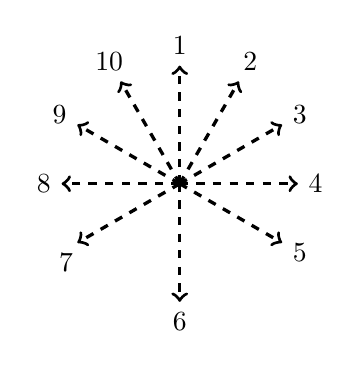
\begin{tikzpicture}
    \setfiguresize{-2.67*\hexxfactor-0.1}{-2.6}{+2.67*\hexxfactor+0.1}{+2.6}
    \begin{scope}
        \drawmediumhexgrid
        \begin{scope}[dashed,very thick, ->]
            \draw (0,0) --   (90:1.5) node [anchor=270] {1};
            \draw (0,0) --   (60:1.5) node [anchor=240] {2};
            \draw (0,0) --   (30:1.5) node [anchor=210] {3};
            \draw (0,0) --    (0:1.5) node [anchor=180] {4};
            \draw (0,0) --  (330:1.5) node [anchor=150] {5};
            \draw (0,0) --  (270:1.5) node [anchor=90 ] {6};
            \draw (0,0) --  (210:1.5) node [anchor=60 ] {7};
            \draw (0,0) --  (180:1.5) node [anchor=0  ] {8};
            \draw (0,0) --  (150:1.5) node [anchor=330] {9};
            \draw (0,0) --  (120:1.5) node [anchor=300] {10};
        \end{scope}
         \drawdotathex{0}{0}
     \end{scope}
\end{tikzpicture}
\end{fitheight}
\hfil
\begin{fitheight}{5.2\standardhexwidth}
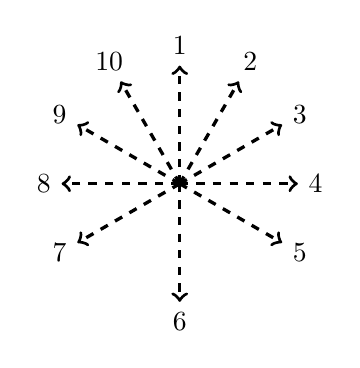
\begin{tikzpicture}
    \setfiguresize{-2.67*\hexxfactor-0.1}{-2.6}{+2.67*\hexxfactor+0.1}{+2.6}
    \begin{scope}[rotate=90]
        \drawmediumhexgrid
        \begin{scope}[dashed,very thick,->]
            \draw (0,0) --   (0:1.5) node [anchor=270] {1};
            \draw (0,0) -- (330:1.5) node [anchor=240] {2};
            \draw (0,0) -- (300:1.5) node [anchor=210] {3};
            \draw (0,0) -- (270:1.5) node [anchor=180] {4};
            \draw (0,0) -- (240:1.5) node [anchor=150] {5};
            \draw (0,0) -- (180:1.5) node [anchor=90 ] {6};
            \draw (0,0) -- (120:1.5) node [anchor=30 ] {7};
            \draw (0,0) --  (90:1.5) node [anchor=0  ] {8};
            \draw (0,0) --  (60:1.5) node [anchor=330] {9};
            \draw (0,0) --  (30:1.5) node [anchor=300] {10};
        \end{scope}
        \drawdotathex{0}{0}
    \end{scope}
\end{tikzpicture}
\end{fitheight}
\hfil
\begin{fitheight}{5.2\standardhexwidth}
\begin{tikzpicture}
    \setfiguresize{-2.67*\hexxfactor-0.1}{-2.6}{+2.67*\hexxfactor+0.1}{+2.6}
    \begin{scope}[rotate=90]
        \miniathex{0.0}{0.5}{\drawmediumhexgrid}
        \begin{scope}[dashed,very thick,->]
            \draw (0,0) --    (0:1.7) node [anchor=270] {1};
            \draw (0:1.000*\hexxfactor) -- +(330:1.0) node [anchor=240] {2};
            \draw (0:0.333*\hexxfactor) --  +(300:1.2) node [anchor=210] {3};
            \draw (0,0) --  (270:1.5) node [anchor=180] {4};
            \draw (180:0.333*\hexxfactor) --  +(240:1.2) node [anchor=150] {5};
            \draw (0,0) --  (180:1.7) node [anchor=90] {6};
            \draw (180:0.333*\hexxfactor) --  +(120:1.2) node [anchor=30 ] {7};
            \draw (0,0) --   (90:1.5) node [anchor=0  ] {8};
            \draw (0:0.333*\hexxfactor) --  +(60:1.2) node [anchor=330] {9};
            \draw (0:1*\hexxfactor) -- +(30:1.0) node [anchor=300] {10};
        \end{scope}
        \drawdotathex{0}{0}
    \end{scope}
\end{tikzpicture}
\end{fitheight}

\x{
\figurecaption{figure:genie-scatter}{AIR-2 Genie Scatter}
}{
\figurecaption{figure:genie-scatter}{Genie Scatter. Roll one die for the direction. Roll another, halving it and rounding down, for the distance.}
}

\end{twocolumnfigure}
}
